\documentclass[12pt]{article}

\usepackage{sbc-template}
\usepackage{graphicx,url}
\usepackage[utf8]{inputenc}
\usepackage[brazil]{babel}
\usepackage{svg}
% \usepackage[latin1]{inputenc}  

\sloppy

\title{Título do Artigo:\\ Subtítulo do artigo}

\author{Dalton Solano dos Reis\inst{1}, Luciana P. de A. Kohler \inst{1}, Marcelo da Silva Hounsell\inst{2} }

\address{Departamento de Sistemas e Computação\\ Universidade Regional de Blumenal (FURB) -- Blumenau, SC -- Brazil
\nextinstitute
  Centro de Ciências Tecnológicas\\ Universidade do Estado de Santa Catarina (UDESC) -- Joinville, SC -- Brazil
\email{\{dalton,Lpa\}@furb.br, marcelo.hounsell@udesc.br}
}

\begin{document} 

\maketitle

\begin{abstract}
  This meta-paper describes the style to be used in articles and short papers for SBC conferences. For papers in English, you should add just an abstract while for the papers in Portuguese, we also ask for an abstract in Portuguese (``resumo''). In both cases, abstracts should not have more than 10 lines and must be in the first page of the paper.
\end{abstract}
     
\begin{resumo} 
  Este meta-artigo descreve o estilo a ser usado na confecção de artigos e resumos de artigos para publicação nos anais das conferências organizadas pela SBC. É solicitada a escrita de resumo e abstract apenas para os artigos escritos em português. Artigos em inglês deverão apresentar apenas abstract. Nos dois casos, o autor deve tomar cuidado para que o resumo (e o abstract) não ultrapassem 10 linhas cada, sendo que ambos devem estar na primeira página do artigo.
\end{resumo}

\section{Informações Gerais}

Todos os artigos completos e pôsteres (artigos curtos) submetidos a algum congresso da SBC, incluindo quaisquer documentos de apoio, devem ser redigidos em inglês ou em português. O formato do artigo deve ser A4, com uma única coluna, margem superior de 3,5 cm, inferior de 2,5 cm e margens laterais de 3,0 cm, sem cabeçalhos ou rodapés. A fonte principal deve ser Times, tamanho nominal 12, com espaçamento de 6 pontos antes de cada parágrafo. A numeração das páginas deve ser suprimida.

Artigos completos devem respeitar os limites de páginas definidos pela conferência. Conferências que publicam apenas resumos solicitam textos de \textbf{uma} página.

\section{Primeira Página} \label{sec:firstpage}

The first page must display the paper title, the name and address of the
authors, the abstract in English and ``resumo'' in Portuguese (``resumos'' are
required only for papers written in Portuguese). The title must be centered
over the whole page, in 16 point boldface font and with 12 points of space
before itself. Author names must be centered in 12 point font, bold, all of
them disposed in the same line, separated by commas and with 12 points of
space after the title. Addresses must be centered in 12 point font, also with
12 points of space after the authors' names. E-mail addresses should be
written using font Courier New, 10 point nominal size, with 6 points of space
before and 6 points of space after.

The abstract and ``resumo'' (if is the case) must be in 12 point Times font,
indented 0.8cm on both sides. The word \textbf{Abstract} and \textbf{Resumo},
should be written in boldface and must precede the text.

\section{Seções e Parágrafos}

Os títulos das seções devem estar em negrito, tamanho 13 pt, alinhados à esquerda. Deve haver um espaço extra de 12 pt antes de cada título. A numeração das seções é opcional. O primeiro parágrafo de cada seção não deve ser indentado, enquanto as primeiras linhas dos parágrafos subsequentes devem ser indentadas em 1,27 cm.

\subsection{Subseção}

O título da subseção deve ser em negrito, 12pt, alinhado à esquerda.

\section{Figuras e Legendas}\label{sec:figs}

As legendas de figuras e tabelas devem ser centralizadas se tiverem menos de uma linha (Figure~\ref{fig:exampleFig1}), caso contrário, devem ser justificadas e com 0,8 cm de recuo em ambas as margens, como mostrado na Figure~\ref{fig:exampleFig2}. A fonte da legenda deve ser Helvetica, tamanho 10, em negrito, com 6 pontos de espaçamento antes e depois de cada legenda.

\begin{figure}[ht]
\centering
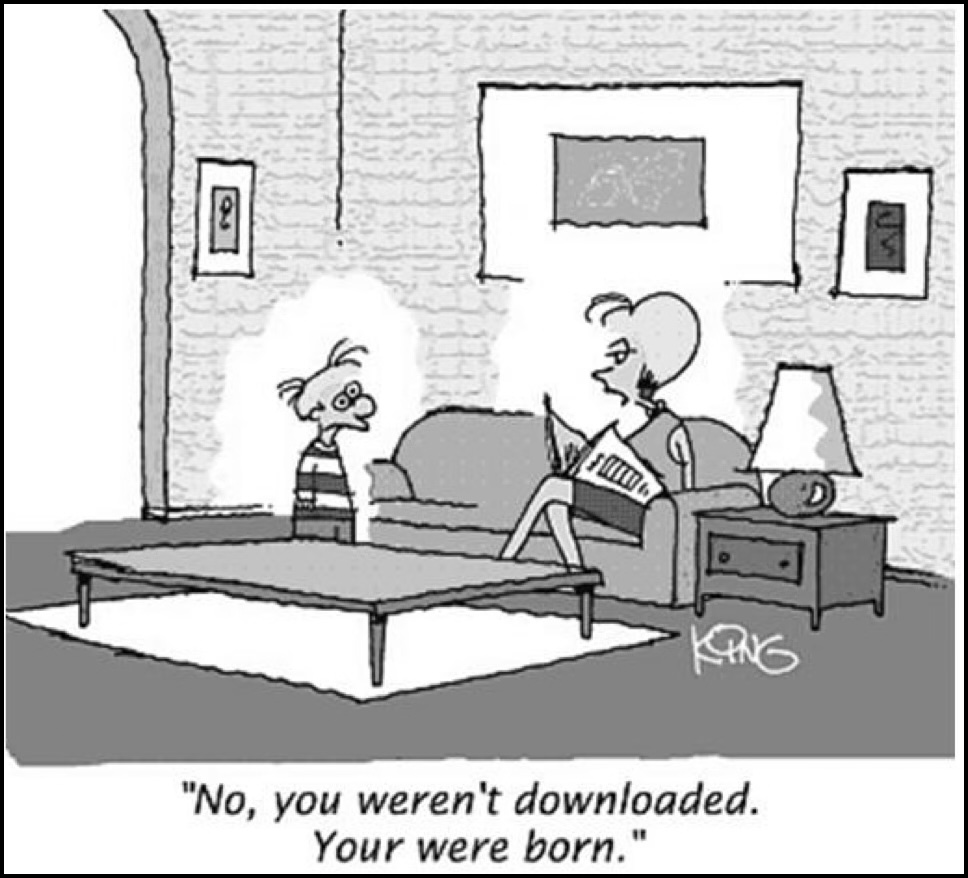
\includegraphics[width=.5\textwidth]{fig1.jpg}
\caption{Uma figura típica}
\label{fig:exampleFig1}
\end{figure}

\begin{figure}[ht]
\centering
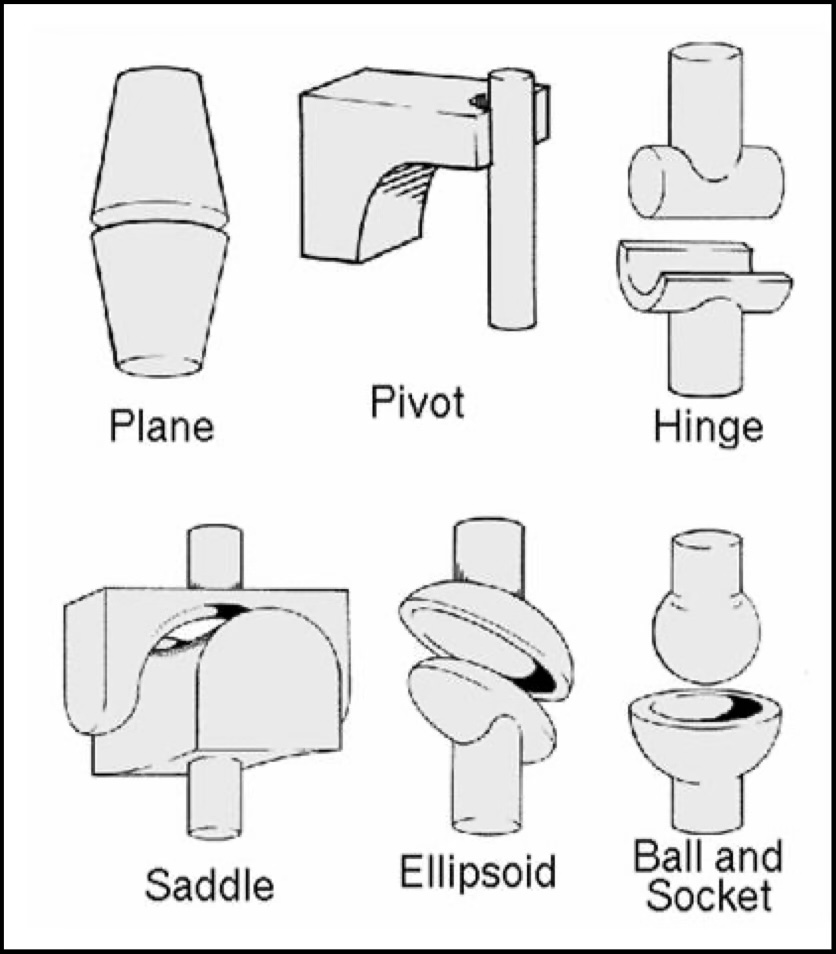
\includegraphics[width=.3\textwidth]{fig2.jpg}
\caption{Esta figura é um exemplo de uma legenda de figura que ocupa mais de uma linha e 
está justificada, considerando os margens mencionados na Seção~\ref{sec:figs}.}
\label{fig:exampleFig2}
\end{figure}

Em tabelas, tente evitar o uso de fundos coloridos ou sombreado, e evite linhas de contorno grossas, duplicadas ou desnecessárias. Ao relatar dados empíricos, não use mais dígitos decimais do que a precisão e reprodutibilidade dos dados exigem. A legenda da tabela deve ser colocada antes da tabela (veja a Tabela 1) e a fonte utilizada deve ser Helvetica, tamanho 10, em negrito, com 6 pontos de espaço antes e depois de cada legenda.

\begin{table}[ht]
  \centering
  \caption{Variáveis a serem consideradas na avaliação das técnicas de interação}
  \label{tab:exTable1}
  \begin{tabular}{|c|c|c|}
    \hline
    \textbf{Cidade} & \textbf{População} & \textbf{Crescimento} \\
    \hline
    Blumenau & 2.123 & 23,56 \\
    Gaspar & 1.340 & 3,40 \\
    Ilhota & 204 & 1,02 \\
    \hline
  \end{tabular}
\end{table}
    
\section{Images}

All images and illustrations should be in black-and-white, or gray tones,
excepting for the papers that will be electronically available (on CD-ROMs,
internet, etc.). The image resolution on paper should be about 600 dpi for
black-and-white images, and 150-300 dpi for grayscale images.  Do not include
images with excessive resolution, as they may take hours to print, without any
visible difference in the result. 

\section{References}

As citações e referências devem seguir as normas da ABNT. Recomendamos que os nomes dos autores sejam dados entre colchetes, por exemplo: \cite{kolevaPropertiesMixedReality1999} e \cite{toriIntroducaoRealidadeVirtual2020}.

As referências devem ser listadas utilizando fonte tamanho 12, com 6 pontos de espaço antes de cada referência. A primeira linha de cada referência não deve ser indentada, enquanto as subsequentes devem ser indentadas por 0,5 cm.

\bibliographystyle{sbc}
\bibliography{../UDESC_RV}

\end{document}
